\section{Introduction}\label{intro}
Machine learning is now an integral part of many software systems for fraud detection, content recognition, automation, and control.
One challenge in developing learning-based applications is that bugs can arise from inconsistent training data, not just faulty code~\cite{sculley2014machine, krishnan2016hilda}.
While developers have several tools at their disposal such as lineage and integrity constraints for classical data processing errors; most of these techniques are difficult to apply directly to learned models.
Linking a prediction on test data to responsible training data is in general uninformative because, in most models, every training example contributes to a prediction in some way.
This challenge is exacerbated by the prevalence of increasingly opaque and high-dimensional models such as Neural Networks, where even considering nearest neighbors might be misleading.
While the database community has made substantial progress in training scalability and model specification~\cite{hellerstein2012madlib,tensor, kraska2013mlbase, crotty2014tupleware, keystone}, the lack of a suitable machine learning analog of data provenance is a critical bottleneck in the development of debugging tools.

As a concrete example, consider designing a control module for self-driving cars using machine learning.
It is unlikely that there is an exhaustive set of training examples for every possible driving condition (e.g., during a once in five years storm).
Consequently, during deployment, the model will have to make predictions for new test data for which there are few similar examples in the training set.
When one of these predictions goes awry, the developer needs to understand: (1) what training data influenced this prediction, (2) how different was this training data from the test example, and (3) whether the differences were due to genuine variation or systematic data inconsistencies.  

\begin{figure}
    \centering
    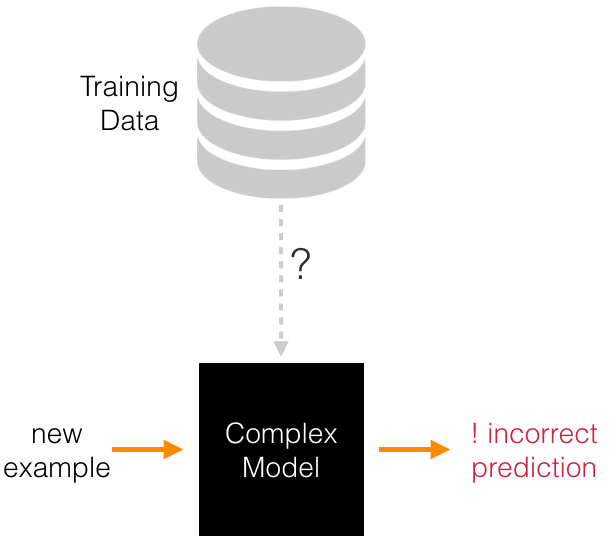
\includegraphics[width=0.48\columnwidth]{figures/teaser1.png}
    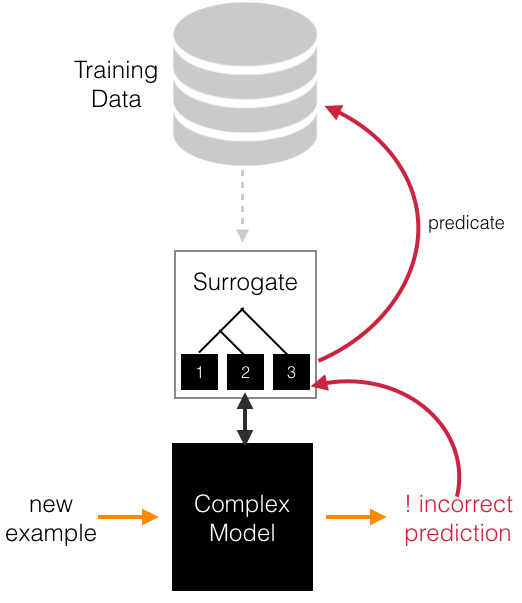
\includegraphics[width=0.48\columnwidth]{figures/teaser2.png}
    \caption{(Left) ML developers need to understand the relationship between training data and a model's predictions, i.e., how are similar points predicted in the training data. But effectively determining the size and range of this neighborhood is challenging in expressive models which can have very complex geometry. (Right) We propose an approximation technique that can represent a black-box model in terms of sub-models applied to feature-space partitions. The developer can quickly determine which data are related based on these partitions.}
    \label{fig:my_label}
\end{figure}

Existing work proposes techniques to enhance model interpretability as one possible solution.
Interpretability can be achieved in two ways: (1) use a simpler, more interpretable model (e.g., a decision tree) from the start, or (2) explain the behavior of a complex model using a simplified approximation~\cite{taylor2016alignment, lei2016rationalizing, ribeiro2016should}. Neither approach is perfect. 
Using a simpler model sacrifices prediction accuracy, which is a trade-off that many model applications are not willing to make.
An example of the second approach is to train a sparse linear model in the local neighborhood of a mispredicted point as a proxy to explain the characteristics (features) that caused the misprediction\cite{taylor2016alignment, lei2016rationalizing, ribeiro2016should}.
Although these approximations can identify salient features, they do not help identify the {\it training data} that led the model towards the misprediction, which might be more useful to a model developer.
This could potentially hide data representation inconsistencies between the training and test data.
Identifying this training data is increasingly important when debugging deep neural network models due to their heavy reliance on large training datasets, which may not always be highly curated and consistent.

We argue that the missing piece is analogous to data provenance in traditional relational or data flow programs, where given an output tuple, the system describes the set of input tuples that cause it to be in the result.
In the case of learning, our objective is to select a set of training data examples that most influence a prediction of a new example.
By influence, we mean that if the labels or features were perturbed for this subset, it would be more likely to change the prediction.
However, for most models, every training data point has some impact on new prediction.
Thus, we simplify the problem to instead identify a {\it sub-partition} of the training data locally approximates the complex model for test points within this sub-partition.  
High-dimensional, non-linear models, such as Neural Networks, have complex decision boundaries, which makes a simple nearest neighbor search unreliable.
Thus, we have to identify a subset of data that aligns with the decision structure of model.

We present \sysfull (\sys), which approximates a complex model (e.g., a deep neural network) using a two-part {\it surrogate model}: a meta-model that partitions the training data, and a set of sub-models that approximate the patterns within each partition.
These sub-models can be arbitrarily complex to capture intricate local patterns. However, the meta-model is constrained to be a decision tree.
This formulation ensures that sub-models are accurate, while the partitions are interpretable as rules.
In contrast to existing model interpretation techniques that return locally relevant features, our approach returns the most informative neighborhood (partition).

Applying \sys to a debugging task is very simple---if a test point is mispredicted, then we can identify the partition it belongs to and investigates that subset of the training data and its associated sub-model.
As our experiments show, the developer can tune the total number of sub-models and the depth of the decision tree to control the trade-off between the specificity of the partitions and how similar the surrogate model is to the complex model.
We anticipate that \sys is a starting point for the developer to further explore the training data and more quickly identify the problematic training data using other visualization or data summarization tools.

The rest of this short paper describes the \sys problem formulation, an algorithm sketch for training surrogate models, as well as an illustration of how \sys can be integrated into a visual model building interface.
Our experiments show that we can generate Fast And Clear Explanations using \sys.
We show that the explanations found by \sys select subsets of data that better align with the structure of the original model than the nearest neighbor or clustering baseline.
Furthermore, we show that \sys is nearly 30x faster than a nearest neighbor query, which is the next most accurate baseline.






